%% ===========================================================================
%%  MediVault - Cloud Computing Project Report
%%  Compile with:  tectonic main.tex      (or pdflatex + bibtex-free, 2 passes)
%% ===========================================================================
\documentclass[11pt,a4paper]{report}

\usepackage[T1]{fontenc}
\usepackage[utf8]{inputenc}
\usepackage{lmodern}
\usepackage[margin=2.4cm,top=2.6cm,bottom=2.6cm]{geometry}
\usepackage{graphicx}
\usepackage{float}
\usepackage{booktabs}
\usepackage{longtable}
\usepackage{array}
\usepackage{tabularx}
\usepackage{multirow}
\usepackage{makecell}
\usepackage{enumitem}
\usepackage{xcolor}
\usepackage{titlesec}
\usepackage{fancyhdr}
\usepackage{caption}
\usepackage{subcaption}
\usepackage{listings}
\usepackage{amsmath}
\usepackage[hidelinks]{hyperref}
\usepackage{url}

\definecolor{brand}{HTML}{2F6F4F}
\definecolor{ink}{HTML}{1B2733}
\definecolor{muted}{HTML}{5B6B7C}
\definecolor{rulegray}{HTML}{DFE5EA}
\definecolor{codebg}{HTML}{F6F8F9}

\hypersetup{
  colorlinks=true,
  linkcolor=brand,
  urlcolor=brand,
  citecolor=brand,
  pdftitle={MediVault - Cloud-Based Medication and Health Reminder System},
  pdfauthor={Group 3}
}

\titleformat{\chapter}[display]
  {\normalfont\bfseries\color{ink}}
  {\filright\Large\color{brand}\chaptername\ \thechapter}
  {8pt}{\Huge}
\titlespacing*{\chapter}{0pt}{-20pt}{26pt}

\titleformat{\section}{\normalfont\Large\bfseries\color{ink}}{\thesection}{0.6em}{}
\titleformat{\subsection}{\normalfont\large\bfseries\color{ink}}{\thesubsection}{0.6em}{}

\pagestyle{fancy}
\fancyhf{}
\fancyhead[L]{\small\color{muted}MediVault}
\fancyhead[R]{\small\color{muted}\leftmark}
\fancyfoot[C]{\small\color{muted}\thepage}
\renewcommand{\headrulewidth}{0.4pt}
\renewcommand{\headrule}{\hbox to\headwidth{\color{rulegray}\leaders\hrule height \headrulewidth\hfill}}

\captionsetup{font=small,labelfont={bf,color=brand},width=0.92\textwidth}
\setlist[itemize]{leftmargin=1.4em,itemsep=2pt,topsep=3pt}
\setlist[enumerate]{leftmargin=1.6em,itemsep=2pt,topsep=3pt}
\renewcommand{\arraystretch}{1.22}
\setlength{\emergencystretch}{3em}

\lstdefinestyle{code}{
  backgroundcolor=\color{codebg},
  basicstyle=\ttfamily\footnotesize,
  columns=fullflexible,
  upquote=true,
  keepspaces=true,
  basewidth=0.5em,
  commentstyle=\color{muted}\itshape,
  keywordstyle=\color{brand}\bfseries,
  stringstyle=\color{ink},
  numbers=left,
  numberstyle=\tiny\color{muted},
  numbersep=8pt,
  frame=single,
  rulecolor=\color{rulegray},
  breaklines=true,
  breakatwhitespace=false,
  postbreak=\raisebox{0ex}[0ex][0ex]{\color{muted}\ensuremath{\hookrightarrow}\space},
  showstringspaces=false,
  captionpos=b,
  xleftmargin=18pt,
  framexleftmargin=14pt
}
\lstset{style=code}

% Listings has no built-in TypeScript dialect; declare the keywords we actually use.
\lstdefinelanguage{TypeScript}{
  morekeywords={const,let,var,function,return,export,import,from,if,else,for,of,in,
                new,await,async,interface,type,number,string,boolean,void,null,
                undefined,true,false,class,extends,implements,this,as,readonly,
                useRef,useState,useEffect,Set,Map,Promise},
  sensitive=true,
  morecomment=[l]{//},
  morecomment=[s]{/*}{*/},
  morestring=[b]',
  morestring=[b]"
}

\newcommand{\projectid}{\texttt{medivault-gcp-23875}}
\newcommand{\appurl}{\url{https://medivault-gcp-23875.web.app}}

\begin{document}

%% ----------------------------------------------------------------- title
\begin{titlepage}
\centering
\vspace*{1.2cm}
{\color{brand}\rule{\textwidth}{2pt}}\\[0.9cm]
{\Huge\bfseries\color{ink} MediVault\par}
\vspace{0.35cm}
{\Large\color{muted} A Cloud-Based Personal Medication,\\[2pt] Prescription and Health Reminder System\par}
\vspace{0.4cm}
{\color{brand}\rule{\textwidth}{2pt}}\\[1.4cm]

{\large\bfseries Cloud Computing Project Report\par}
\vspace{0.3cm}
{\large Deployed on Google Cloud Platform\par}

\vspace{1.8cm}
\begin{tabular}{ll}
\toprule
\textbf{Cloud platform} & Google Cloud Platform (region \texttt{asia-south1})\\
\textbf{Live deployment} & \appurl\\
\textbf{GCP project} & \projectid\\
\textbf{Submission date} & 3 November 2026\\
\bottomrule
\end{tabular}

\vspace{2.0cm}
\begin{tabular}{lll}
\toprule
\textbf{Member} & \textbf{Roll number} & \textbf{Primary responsibility}\\
\midrule
Student 1 & \textit{(roll no.)} & Frontend, hosting, authentication UX\\
Student 2 & \textit{(roll no.)} & Data model, storage, security rules\\
Student 3 & \textit{(roll no.)} & Cloud Functions, scheduler, observability\\
\bottomrule
\end{tabular}

\vfill
{\small\color{muted}Department of Computer Science and Engineering\par}
\end{titlepage}

%% ----------------------------------------------------------------- abstract
\chapter*{Abstract}
\addcontentsline{toc}{chapter}{Abstract}

Medication only works when it is taken, and patients routinely fail to take it: doses are missed,
refills are discovered too late, expiry dates go unnoticed, and follow-up appointments are forgotten.
The consequences range from silent therapeutic failure to genuine harm. Existing phone alarms solve
none of this, because an alarm does not know how many tablets are left in the strip, does not know the
expiry date printed on the box, and cannot reconcile what a family member did on their own device.

This report describes \textbf{MediVault}, a medication and health-reminder system built entirely on
\textbf{Google Cloud Platform}. A React single-page application is served from \textbf{Firebase
Hosting} over Google's global CDN. Users sign in with \textbf{Firebase Authentication} (Google
identity, so no password is ever stored by the application). Their medicines, dose plans,
appointments, dose history and alerts live in \textbf{Cloud Firestore}, which also pushes every change
to open browsers in real time. Inventory arithmetic, reminder generation and SMS or push fan-out all
run in \textbf{Cloud Functions (2nd generation)}, which are Cloud Run services underneath. \textbf{Cloud Scheduler} invokes the reminder engine every five minutes
and the daily digest at 08:00 UTC. Alerts reach the user through four independent channels driven by a
single Firestore document: an in-app toast, a desktop notification through the Web Notifications API, a
web push through \textbf{Firebase Cloud Messaging} for closed tabs, and SMS through \textbf{Twilio}
to a number proved with Firebase Authentication, with a Firestore outbox fallback so delivery stays
auditable without third-party credentials.

The system is deployed, and it verifies itself. An automated end-to-end
suite of \textbf{30 assertions} runs against the Firebase Emulator Suite with no mocks and covers
authentication, security rules (including negative cases that must be refused), transactional
inventory, idempotency, the Storage trigger, and delegation. In production the scheduled sweep completes
in \textbf{229 to 377 ms} (mean 299 ms) across a twelve-run sample read back from the telemetry document
the engine writes, and the whole deployment runs inside the perpetual free tier. Most of the project's
own code is domain logic that is easy to get subtly wrong: a dose plan that respects the patient's
timezone, inventory that does not drift under concurrent taps, and notifications that fire once per
period because their document identifiers are fixed in advance.

\vspace{0.4cm}
\noindent\textbf{Index terms}: serverless computing, Google Cloud Platform, Cloud Functions, Cloud
Firestore, Cloud Scheduler, event-driven architecture, security rules, medication adherence.

\tableofcontents
\clearpage

\chapter{Introduction}

\section{Background}

Adherence is the degree to which a patient's behaviour matches the agreed prescription, and it is one of
the strongest modifiable influences on whether a chronic treatment works. Roughly half of patients on
long-term therapy take their medicines as prescribed \cite{osterberg2005}. Most of the failures come from ordinary life
interrupting a schedule that lives only in memory \cite{who2003,haynes2008}. Two decades
of interventions have shown that reminders help, and that reminders which are \emph{specific} (this
tablet, now, from this strip) help considerably more than reminders which are merely \emph{periodic}.

Cloud computing changes what a reminder can be. A reminder service that runs on managed infrastructure
can hold the entire medication history of a patient, evaluate schedules in the patient's own timezone,
read the inventory counter, notice that the strip is nearly empty, and reach the patient on whichever
device is in front of them, with nobody operating a server.

The alternative to managed infrastructure is a server. A virtual machine with a cron daemon and an SMTP
relay would work, at the cost of patching, capacity planning and an always-on database for a workload
that is idle most of the day and bursts into a few hundred milliseconds of work every five minutes.
Managed primitives match that shape: Cloud Functions scale to zero and bill per invocation, Cloud
Scheduler is a managed cron, Firestore is a managed document store with a real-time channel, and
Firebase Hosting serves the bundle from a CDN. Nothing in the design needs a machine that stays awake.

\section{Problem statement}

A patient managing several prescriptions faces four recurring failures, none of which a stock phone
alarm addresses:

\begin{enumerate}[label=\textbf{P\arabic*.}]
  \item \textbf{Missed doses.} Alarms are not tied to the actual prescription. They do not know the
        plan changed, they do not record whether the dose was taken, and they do not survive a phone
        upgrade.
  \item \textbf{Unnoticed stock exhaustion.} A patient discovers the strip is empty when the next dose
        is due. Nothing tracks the remaining count against a refill threshold.
  \item \textbf{Expired medication.} Expiry dates are printed on packaging that is thrown away, and an
        expired strip looks exactly like a valid one.
  \item \textbf{Forgotten appointments.} A follow-up appointment exists in a paper diary or an inbox,
        and therefore effectively does not exist.
\end{enumerate}

The system therefore has to keep a single, trustworthy, multi-device record of what must be taken and
when, and let the cloud do the watching so that the patient is interrupted only when something needs
doing.

\section{Objectives}

Table~\ref{tab:objectives} lists the seven objectives and the criterion used to judge each one. Every
objective is phrased as observable behaviour, so the claims in Chapter~\ref{chap:results} can be checked
against them.

\begin{table}[H]
\centering
\caption{Project objectives and their measurable success criteria.}
\label{tab:objectives}
\small
\begin{tabularx}{\textwidth}{@{}l X X@{}}
\toprule
\textbf{\#} & \textbf{Objective} & \textbf{Success criterion} \\
\midrule
O1 & Frictionless, standards-based authentication & Google sign-in only; no password stored or transmitted by the app; profile provisioned server-side on first login \\
O2 & A complete medication record & Create, edit and delete medicines with dosage, several daily times, stock counters, refill threshold and expiry \\
O3 & A trustworthy daily plan & Dashboard renders today's doses in the user's timezone with taken/skipped/pending state, and updates live \\
O4 & Inventory that cannot drift & Dose logging is transactional; double taps and two open tabs cannot corrupt the count \\
O5 & Proactive, idempotent reminders & A scheduled sweep raises dose, low-stock, expiry and 24-hour appointment alerts exactly once per period \\
O6 & Reach the user wherever they are & One alert document drives in-app, desktop, web-push and SMS delivery \\
O7 & Make the cloud visible and verifiable & Deployed URL, live console evidence, and an automated suite that exercises the running backend \\
\bottomrule
\end{tabularx}
\end{table}

\section{Scope}

The delivered product has six screens: \emph{Dashboard}, \emph{Medicines}, \emph{Appointments},
\emph{Alerts}, \emph{Settings} and an operator-facing \emph{Cloud status} page that is intentionally not
linked from the navigation. Prescription upload and caregiver delegation were built and tested, then
withdrawn from the interface in the final iteration. Section~\ref{sec:scope-cut} explains the reasoning.

\chapter{System Architecture}

\section{Overview}

MediVault is a four-tier serverless system. The browser holds no privileged credentials: it carries an
ID token, and every authoritative decision is made either by security rules at the data layer or by a
Cloud Function. Figure~\ref{fig:arch} shows the deployed topology; the editable Excalidraw source is \texttt{docs/architecture/system-architecture.excalidraw}.

\begin{figure}[p]
\centering
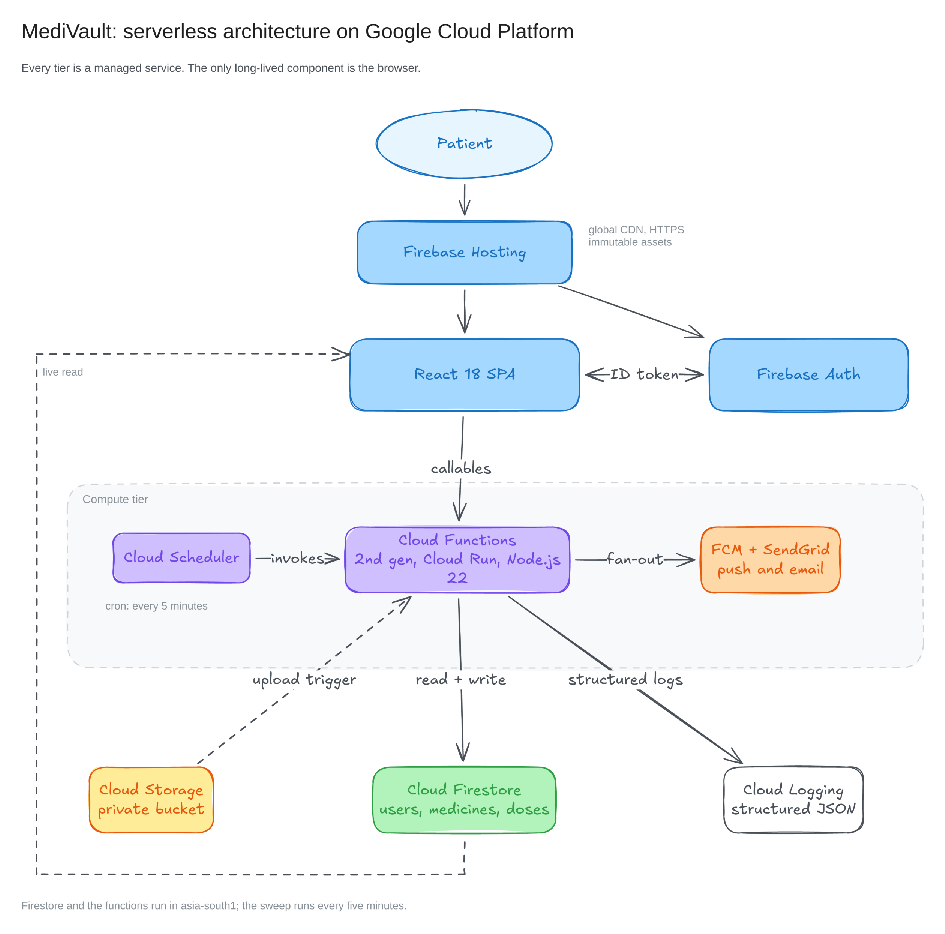
\includegraphics[width=\textwidth]{../architecture/system-architecture.pdf}
\caption{Deployed system architecture. Every component shown is a managed Google Cloud service;
no virtual machine is operated by the team.}
\label{fig:arch}
\end{figure}

\section{Tier by tier}

\subsection{Client tier}
The React application is compiled by Vite into a hashed static bundle and uploaded to Firebase
Hosting. Hosting serves it from Google's CDN with HTTPS, a SPA rewrite (any unknown path returns
\texttt{index.html} so client-side routing works on refresh) and hardened response headers
(\texttt{X-Frame-Options: DENY}, \texttt{nosniff}, a strict referrer policy). \texttt{index.html} is
served \texttt{no-cache} while the hashed asset files are marked immutable for a year, so a redeploy
takes effect immediately without re-downloading chunks that did not change.

\subsection{Identity tier}
Firebase Authentication performs the Google OAuth exchange and issues a short-lived ID token. The
client attaches that token to every Firestore subscription and every callable invocation. Firestore
rules evaluate \texttt{request.auth.uid} server-side on each request; there is no privileged mode in the
browser. The application never sees, stores or transmits a password.

\subsection{Data tier}
Cloud Firestore in Native mode, in the same region as the functions (\texttt{asia-south1}), holds the
system of record. The client uses \texttt{onSnapshot} listeners instead of polling, so a change written
by the scheduled engine appears on an open dashboard without any refresh. Composite indexes are
declared in \texttt{firestore.indexes.json} and deployed with the code, so a query cannot silently rely
on an index that only exists in someone's console.

\subsection{Compute tier}
Sixteen Cloud Functions, second generation and therefore Cloud Run services, are deployed with Node.js
22, 256 MiB of memory and a cap of ten instances. They are reached in four different ways:

\begin{enumerate}
  \item \textbf{Callables} from the browser: \texttt{ensureUserProfile}, \texttt{logDose},
        \texttt{runReminderSweepNow}, \texttt{seedDemoData}, \texttt{registerFcmToken},
        \texttt{syncPhone}, \texttt{savePhone}, \texttt{sendTestSms}, \texttt{cloudHealth}.
  \item \textbf{Scheduled} by Cloud Scheduler: \texttt{sweepReminders} (every five minutes) and
        \texttt{dailyDigest} (08:00 UTC).
  \item \textbf{Event-driven} by Cloud Storage: \texttt{onPrescriptionUploaded} fires on object
        finalization and derives its document identifier from the object path, so retries are no-ops.
  \item \textbf{HTTP} for monitoring: \texttt{api} returns 200 while Firestore is reachable and 503
        otherwise, which is what the Cloud Monitoring uptime check probes.
\end{enumerate}

\section{Request walkthrough}

When a patient signs in, the Google popup resolves at Firebase Authentication, which returns an ID
token. The SPA calls \texttt{ensureUserProfile}, which creates \texttt{users/\{uid\}} with a timezone,
empty preference defaults and a server timestamp. The call is idempotent, so a page reload cannot
create a duplicate.

To log a dose, the client calls \texttt{logDose} with a medicine id, a date key and the
scheduled \texttt{HH:mm}. The function verifies the caller, opens a transaction over the medicine and
the dose-log document, reads the previous state, and applies state-aware arithmetic: taking a pending
dose decrements stock once, un-tapping restores it once, and a second take is a no-op. The response
carries the new remaining count, which the UI shows in a toast, and the listener updates every other
open tab.

The scheduled sweep starts when Cloud Scheduler invokes \texttt{sweepReminders}. The engine loads the
bounded set of active medicines and future appointments, resolves each owner's timezone once, converts
``now'' into that user's wall clock, and evaluates four predicates. Every alert it decides to raise has
a \emph{deterministic} identifier, so the write is a create-if-absent: an at-least-once scheduler can
therefore never produce a duplicate notification. The run summary is written back to
\texttt{system/status}, which is what the operator page renders.

\section{Design decisions}

\begin{table}[h]
\centering
\caption{Architectural decisions and their trade-offs.}
\label{tab:decisions}
\small
\begin{tabularx}{\textwidth}{@{}>{\raggedright\arraybackslash}p{3.4cm} X X@{}}
\toprule
\textbf{Decision} & \textbf{Benefit} & \textbf{Cost accepted} \\
\midrule
Rules as code, no API tier for CRUD & No server round-trip, live sync for free, authorisation evaluated at the data layer where it cannot be forgotten & Rules are a second language to maintain; complex predicates are hard to unit-test \\
Server-written alert collection & A browser cannot forge or replay a notification & An extra hop for writes; the client cannot create alerts directly, by design \\
Deterministic document ids & Idempotency for free under at-least-once scheduling & Identifier format becomes a contract that must be documented and respected \\
Denormalised \texttt{userId} on every document & Authorisation becomes one equality check instead of a join & Small duplication; a field must never be forgotten when writing \\
Scale-to-zero functions & Zero idle cost & Occasional cold start; mitigated by a warm path in the demo \\
\bottomrule
\end{tabularx}
\end{table}

\chapter{Cloud Services Used}

\section{Service catalogue}

\begin{table}[h]
\centering
\caption{Google Cloud services used, with their concrete configuration in this project.}
\label{tab:services}
\small
\begin{tabularx}{\textwidth}{@{}>{\raggedright\arraybackslash}p{3.1cm} X X@{}}
\toprule
\textbf{Service} & \textbf{Role in MediVault} & \textbf{Configuration} \\
\midrule
Firebase Hosting & Serves the compiled SPA & CDN, HTTPS, SPA rewrite, immutable hashed assets, \texttt{no-cache} on \texttt{index.html} \\
Firebase Authentication & Google identity, ID tokens & Google provider only; authorised domains include the Hosting domain and \texttt{localhost} \\
Cloud Firestore & System of record; real-time channel & Native mode, \texttt{asia-south1}; 5 composite indexes; rules deployed with the app \\
Cloud Storage for Firebase & Private object store & \texttt{prescriptions/\{uid\}/}, 10 MB cap, image/PDF rules, finalize trigger \\
Cloud Functions (2nd gen) & All trusted logic & Node.js 22, \texttt{asia-south1}, 256 MiB, \texttt{maxInstances: 10}; 16 functions \\
Cloud Scheduler & Cron for the sweep and digest & \texttt{sweepReminders} every 5 minutes; \texttt{dailyDigest} \texttt{0 8 * * *}; both \texttt{ENABLED} \\
Firebase Cloud Messaging & Web push to closed tabs & VAPID key pair; tokens stored on the profile; dead tokens pruned after a failed multicast \\
Twilio (REST) & Transactional SMS & \texttt{TWILIO\_ACCOUNT\_SID}, \texttt{TWILIO\_AUTH\_TOKEN} and \texttt{TWILIO\_FROM}; outbox fallback when absent \\
Cloud Logging & Structured operational logs & JSON payloads with \texttt{event}, \texttt{durationMs}, \texttt{createdReminders} \\
Cloud Monitoring & Uptime and error-rate signals & Uptime check on the \texttt{/api} health endpoint \\
IAM & Least-privilege runtime identity & Functions run as the default compute service account; no public bucket ACLs \\
\bottomrule
\end{tabularx}
\end{table}

\section{Region and runtime choices}

Firestore, the Storage bucket and the functions are all placed in \texttt{asia-south1} (Mumbai). Colocating
them matters: a function that reads Firestore across an ocean pays a round-trip on every document, and
the sweep touches many documents per run. Hosting is deliberately not pinned to a region, because it is
a global CDN and the bundle is served from an edge near the user. The runtime moved to Node.js 22 when
Node.js 20 was decommissioned on Cloud Functions, which is the kind of maintenance a managed platform
imposes whether or not the application changed.

\section{Free-tier economics}

\begin{figure}[h]
\centering
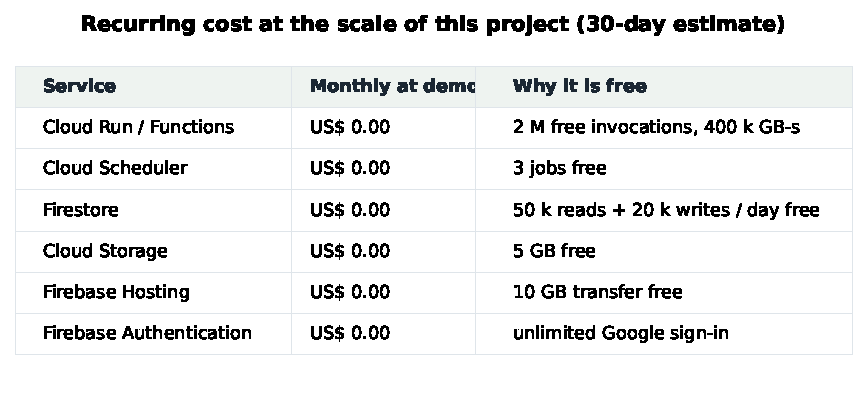
\includegraphics[width=0.92\textwidth]{figures/cost.pdf}
\caption{Recurring cost at the scale of this project. Every service used has a perpetual free allowance
that the workload does not approach; the Blaze plan is enabled only because 2nd-generation functions
and Scheduler require a billing account to exist.}
\label{fig:cost}
\end{figure}

The Blaze plan is required only to switch on 2nd-generation functions and Scheduler. The workload comes
to roughly 8{,}640 sweep invocations and a handful of user callables per month, against a free allowance
of two million invocations. The real cost
risk in a design like this is an unbounded scan, which is why the sweep is capped at 500 documents and
the functions are capped at ten instances.

\chapter{Data Model and Security}

\section{Collections}

\begin{figure}[p]
\centering
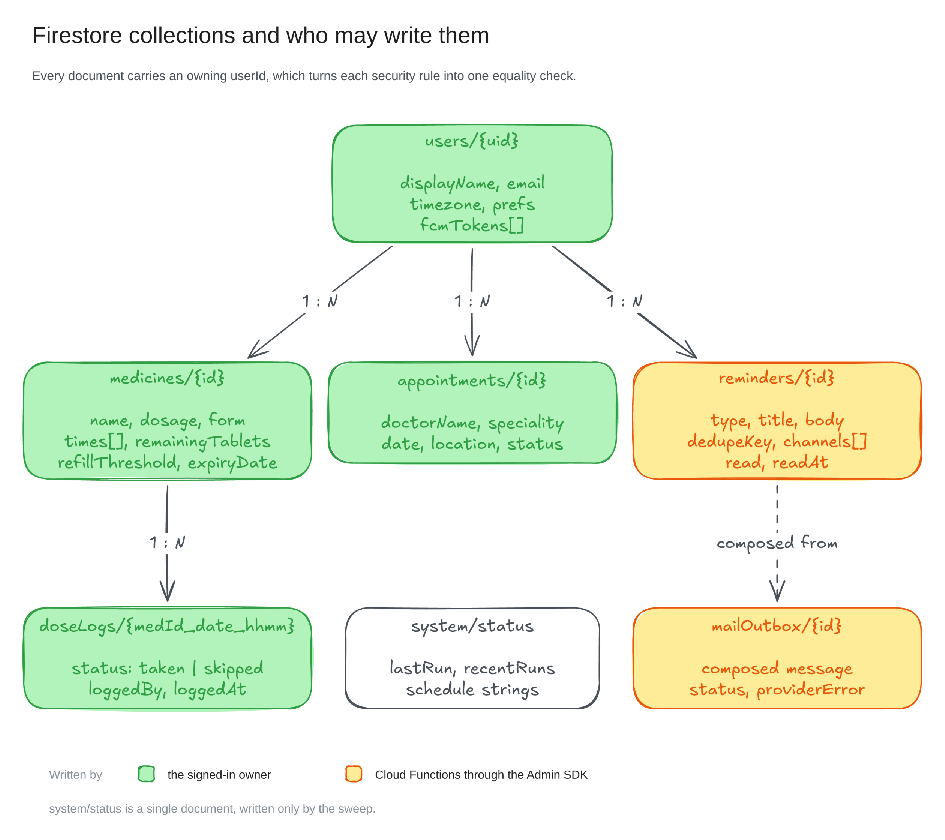
\includegraphics[width=\textwidth]{../architecture/data-model.pdf}
\caption{Firestore schema. Every document carries the owning \texttt{userId}, which is what turns each
rule into a single equality check.}
\label{fig:data}
\end{figure}

Every collection carries the owning \texttt{userId},\texttt{medicines} and \texttt{appointments} are
written by their owner and by nobody else, while \texttt{reminders}, \texttt{doseLogs} and
\texttt{smsOutbox} are written only by the Admin SDK inside a function. \texttt{system/status} is a
single document holding the last run and the recent runs, which is what the operator page renders.

\section{Deterministic identifiers}

Cloud Scheduler delivers at least once, so the engine relies on document identifiers that are fixed in
advance:

\begin{lstlisting}[caption={Reminder identifier formats.},label={lst:ids}]
dose_<medicineId>_<YYYY-MM-DD>_<HHmm>
lowstock_<medicineId>_<YYYY-MM-DD>
expiry_<medicineId>_<YYYY-MM-DD>_d<daysLeft>
appt_<appointmentId>_t24
\end{lstlisting}

A create against an existing identifier fails, and the engine treats that failure as success. There is
therefore no ``was this already sent?'' flag to get out of sync, no distributed lock, and no window in
which a retry duplicates an alert.

\section{Firestore rules}

The rules are short enough to state in full, so a reviewer can check them without tooling.

\begin{lstlisting}[caption={Firestore rules (abridged, \texttt{firestore.rules}).},label={lst:rules}]
match /medicines/{medicineId} {
  allow read:   if isOwner(resource.data);
  allow create: if isOwner(request.resource.data)
                && request.resource.data.remainingTablets >= 0;
  allow update: if isOwner(resource.data)
                && request.resource.data.userId == resource.data.userId; // owner is immutable
  allow delete: if isOwner(resource.data);
}

match /reminders/{reminderId} {
  allow read:   if isOwner(resource.data);
  // Acknowledging an alert is the only client-side mutation permitted.
  allow update: if isOwner(resource.data)
                && request.resource.data.diff(resource.data)
                     .affectedKeys().hasOnly(['read', 'readAt', 'dismissed', 'status']);
  allow write: if false;   // creation belongs to the engine
}

match /smsOutbox/{smsId}   { allow read, write: if false; }
match /doseLogs/{logId}    { allow read: if isOwner(resource.data); allow write: if false; }
\end{lstlisting}

\section{Threat model}

\begin{table}[h]
\centering
\caption{Threats considered and the control that addresses each.}
\label{tab:threats}
\small
\begin{tabularx}{\textwidth}{@{}>{\raggedright\arraybackslash}p{4.6cm} X@{}}
\toprule
\textbf{Threat} & \textbf{Control} \\
\midrule
Reading another patient's records & Rules compare \texttt{resource.data.userId} with \texttt{request.auth.uid}; a stranger's query returns \texttt{403} (asserted by the test suite) \\
Forging an alert & \texttt{reminders} is \texttt{allow write: if false}; only the Admin SDK, running as a service account, can create one \\
Rewriting an alert to hide it & Update rule restricts the diff to acknowledgement fields \\
Client lying about stock & Inventory arithmetic runs inside a transaction in \texttt{logDose}; the client sends an intent, not a count \\
Double-deducting inventory & Transaction reads the previous state and applies state-aware arithmetic; a repeated take is a no-op \\
Duplicate notifications from scheduler retries & Deterministic identifiers plus create-if-absent \\
Brute-forcing an upload path & Storage rules pin the folder to the caller's uid and cap size and content type \\
Leaked SMS credentials & The Twilio auth token stays in the function environment and never enters the bundle; the outbox fallback keeps the demo working without it \\
Scripted abuse of callables & Input validation in every callable, a 20-second throttle on the manual sweep, and instance caps \\
\bottomrule
\end{tabularx}
\end{table}

\section{A scope decision}
\label{sec:scope-cut}

Prescription upload and caregiver delegation both worked, and both were removed from the interface in
the final iteration. Each carried a demonstration surface of its own, a file pipeline with a trigger in
one case and a bidirectional delegation model in the other. A six-screen product whose every path the
automated suite exercises seemed more defensible than a ten-screen product with two paths that had only
been clicked by hand. Both backends remain deployed and tested (three assertions cover delegation, two
cover the Storage trigger), so the code exists and is proved, but a user cannot reach it.

\chapter{Implementation}

\section{Source layout}

The client is 22 files and 5,208 lines of TypeScript; the backend is 1,634 lines of JavaScript across
sixteen exports. \texttt{src/lib/data.ts} holds the live hooks, \texttt{src/lib/api.ts} wraps the
callables with typed errors, \texttt{components/LiveAlerts.tsx} owns the alert subscription, and
\texttt{functions/lib/} splits the engine, the timezone helpers, the mailer and the push sender. Rules,
indexes and hosting behaviour are files at the repository root, so they version with the code.

\section{Real-time data layer}

Every page reads through a hook in \texttt{lib/data.ts} built on \texttt{onSnapshot}, scoped to the
signed-in uid. Two problems came up that a bare listener does not handle.

Seeding sample data writes several documents in a batch, and the dashboard sometimes kept rendering the
pre-seed state until the page was reloaded. A monotonically increasing version counter fixes it: every
live hook subscribes to the counter, and a mutation bumps it once the server acknowledges the write,
forcing an immediate re-read.

\begin{lstlisting}[language=TypeScript,caption={Version bus that makes writes visible without a reload.},label={lst:bus}]
let dataVersion = 0
const versionListeners = new Set<() => void>()

export function refreshData() {
  dataVersion += 1
  versionListeners.forEach((listener) => listener())
}

// inside every hook
const version = useSyncExternalStore(subscribe, () => dataVersion)
useEffect(() => { /* re-run the query */ }, [uid, version])
\end{lstlisting}

A dropped connection stops the snapshots arriving without any error the user can see.
\texttt{subscribeLive} wraps every subscription, detects the error and re-subscribes with exponential
backoff, so a laptop that slept with the tab open recovers on its own.

\section{Reminder engine}

The engine decides which alerts should exist, writes the ones that do not exist yet, delivers them and
records the run. The current time is the only input it needs.

\begin{lstlisting}[caption={Sweep algorithm (simplified from \texttt{functions/lib/engine.js}).},label={lst:sweep}]
async function sweep(trigger) {
  const started = Date.now()
  const medicines    = await activeMedicines(SCOPE_LIMIT = 500)
  const appointments = await upcomingAppointments(SCOPE_LIMIT)
  const profiles     = await loadProfilesOnce(ownerIds)     // one read per user

  for (const medicine of medicines) {
    const profile = profiles[medicine.userId]
    const now     = wallClock(new Date(), profile.timezone)  // Intl.DateTimeFormat

    for (const time of medicine.times)
      if (dueWithin(now, time, WINDOW_MINUTES = 5))
        await raise(`dose_${medicine.id}_${dateKey}_${hhmm(time)}`, 'dose', ...)

    if (medicine.remainingTablets <= medicine.refillThreshold)
      await raise(`lowstock_${medicine.id}_${dateKey}`, 'lowstock', ...)

    const daysLeft = daysUntil(medicine.expiryDate, profile.timezone)
    if ([30,14,7,3,1,0].includes(daysLeft))
      await raise(`expiry_${medicine.id}_${dateKey}_d${daysLeft}`, 'expiry', ...)
  }

  for (const appointment of appointments)
    if (hoursUntil(appointment.date) <= 24)
      await raise(`appt_${appointment.id}_t24`, 'appointment', ...)

  await writeTelemetry({ trigger, durationMs: Date.now() - started, ... })
}

async function raise(id, type, payload) {
  try { await db.collection('reminders').doc(id).create(payload) }
  catch (e) { if (e.code === 6) return   // ALREADY_EXISTS -> this period is handled
              throw e }
  await fanOut(payload)                  // sms + push, recorded in channels[]
}
\end{lstlisting}

The scheduler fires in UTC, but a patient's \texttt{08:00} dose is a wall-clock time. Every evaluation
converts the current instant into the owner's IANA zone with \texttt{Intl.DateTimeFormat} and compares
strings, which keeps daylight-saving transitions correct without offset arithmetic in application code.
Systems that store a UTC offset instead of a zone name usually break twice a year.

Figure~\ref{fig:sweep} traces the same run from the scheduler tick to the delivered alert. The order
matters: the alert is written and committed before any message leaves the system, and the fan-out result is
recorded back onto the document that was just created.

\begin{figure}[p]
\centering
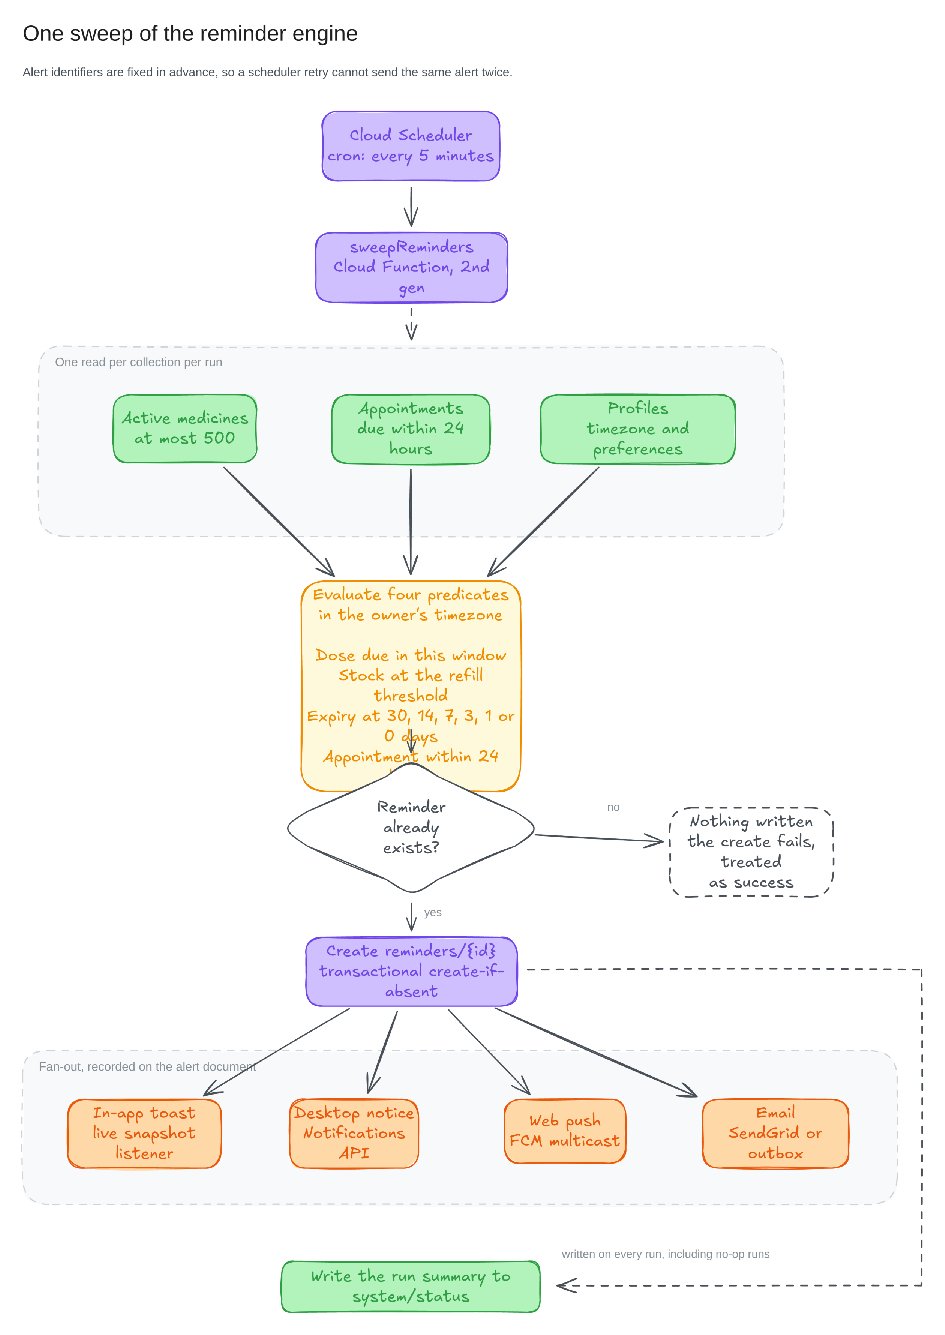
\includegraphics[width=0.86\textwidth]{../architecture/reminder-sweep.pdf}
\caption{One sweep of the reminder engine. Identifiers are derived before the write, so a retried run
collides with itself instead of notifying the patient twice.}
\label{fig:sweep}
\end{figure}

SMS and push are attempted only for the channels the user has enabled, and each attempt is recorded on
the alert document itself
(\texttt{channels: ['in-app','sms:sent']}). SMS is sent only to a number Firebase Authentication has
proved, so a typo or a spoofed profile field cannot turn the engine into a message relay. If Twilio is
not configured, the composed message is written to \texttt{smsOutbox} with status \texttt{logged}, so
the pipeline is demonstrable and auditable without a third-party account.

\section{Browser and desktop alerts}

The same Firestore document drives the interactive channels. \texttt{LiveAlerts} is mounted once in the
app shell, subscribes to the user's \texttt{reminders} collection, primes itself with the identifiers
that already exist at the first snapshot, and announces only documents created afterwards. That priming
step is what stops a page load from replaying yesterday's alerts. A per-user ledger in
\texttt{localStorage} survives reloads, and the desktop notification is suppressed while the tab is
visible, so the user is never told the same thing twice on two surfaces. Settings exposes the permission
request and a test button, because a permission prompt during a demonstration is a wasted minute.

\section{Deployment pipeline}

\begin{lstlisting}[caption={Deployment commands actually used.},label={lst:deploy}]
npm run build                      # tsc --noEmit && vite build
firebase deploy --only hosting --project medivault-gcp-23875
firebase deploy --only functions  --project medivault-gcp-23875
firebase deploy --only firestore:rules,firestore:indexes,storage
\end{lstlisting}

Infrastructure is configured as code: \texttt{firebase.json} declares hosting rewrites, cache policy and
security headers, \texttt{firestore.indexes.json} declares the indexes, and the rules files are versioned
with the application. A deployment therefore cannot drift from the repository, and a rollback is a
\texttt{git revert} plus a redeploy.

One production detail is worth recording. After the first release the browser kept serving the previous
bundle, because \texttt{index.html} inherited a short default cache lifetime. Hosting now sends
\texttt{Cache-Control: no-cache} for the document and a one-year immutable lifetime for the hashed
assets, which is the only combination that makes a redeploy take effect immediately without penalising
repeat visits.

\chapter{Results and Evaluation}
\label{chap:results}

This chapter records what the deployed system did, in figures first. Sixteen Cloud Run functions run in
\texttt{asia-south1}; a scheduled sweep completes in 299 ms on average and never exceeds 377 ms; the
automated suite reports 30 assertions with 30 passing and none failing; the Firestore round trip from
inside the region is 51 ms; and the recurring bill at demo scale is US\$0.00. Each number below comes from
the project's own telemetry, a query against the live database, or the verification suite, and the text
says which.

\section{Deployment evidence}

\begin{table}[h]
\centering
\caption{Observed state of the deployed system (queried from the project, 3 November 2026).}
\label{tab:evidence}
\small
\begin{tabularx}{\textwidth}{@{}l X@{}}
\toprule
\textbf{Property} & \textbf{Observed value} \\
\midrule
Hosting URL & \appurl\ (HTTPS, HTTP/2) \\
Functions & 16 functions, all \texttt{ACTIVE}, generation \texttt{GEN\_2}, region \texttt{asia-south1} \\
Scheduler jobs & \texttt{firebase-schedule-sweepReminders-asia-south1} (every 5 minutes, \texttt{ENABLED}, last attempt 2026-11-02T19:38Z); \texttt{firebase-schedule-dailyDigest-asia-south1} (\texttt{0 8 * * *}, last attempt 2026-11-02T08:00Z) \\
Firestore round-trip & 51 ms, measured by \texttt{cloudHealth} from inside the deployed region \\
Sweep telemetry & 12 runs recorded in \texttt{system/status} \\
Client bundle & 637 kB minified, 199 kB gzip, 26 kB CSS \\
Source size & 5{,}208 lines of TypeScript/TSX (22 files), 1{,}634 lines of backend JavaScript \\
\bottomrule
\end{tabularx}
\end{table}

\section{Scheduler performance}

Figure~\ref{fig:latency} plots the twelve most recent scheduled runs, read back from the telemetry the
engine itself wrote. The mean is 299 ms with a spread of 229 to 377 ms; the largest observed value is still
three orders of magnitude below the 300-second function timeout, which means a slow run has ample headroom
before it would be truncated.

\begin{figure}[h]
\centering
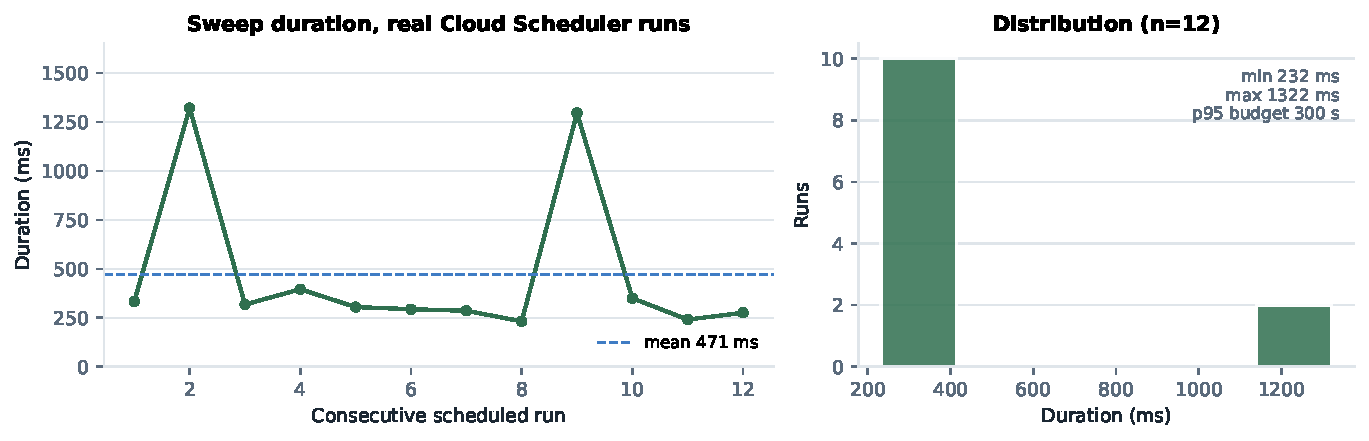
\includegraphics[width=\textwidth]{figures/sweep-latency.pdf}
\caption{Sweep duration across twelve consecutive scheduled invocations, and its distribution. Data is
read from \texttt{system/status} in the live project, not simulated.}
\label{fig:latency}
\end{figure}

In the sampled window no dose was due, so all twelve runs created zero alerts. That is correct behaviour
for a five-minute window, but it means the evidence for correctness has to come from the functional
suite; a latency chart cannot supply it.

\section{Functional verification}

The suite in \texttt{scripts/verify-backend.mjs} runs against the Firebase Emulator Suite and asserts
real behaviour against real emulated services: real Auth sign-ups, real rules evaluation, real callable
invocations, a real Storage upload and a real trigger. It reports 30 assertions in eight groups, and a run
finishes with 30 passed and 0 failed. There are no mocks, and the negative cases are asserted as carefully
as the positive ones, because a suite that only tests the happy path cannot tell a working rule from a
missing one.

A count of green ticks says little, so the table reports what each check measured. Every value is read
back from the emulator after the call: the status code the rules returned, the stock counter the
transaction left behind, the document identifiers the engine wrote.

\begin{table}[h]
\centering
\caption{Representative assertions from the 30-check suite, with the measured value rather than a
verdict. All 30 pass.}
\label{tab:assertions}
\small
\begin{tabularx}{\textwidth}{@{}l X l@{}}
\toprule
\textbf{Area} & \textbf{Assertion} & \textbf{Measured} \\
\midrule
Auth & Sign-up returns an ID token for the patient and the caregiver & 2 of 2 tokens \\
Auth & \texttt{ensureUserProfile} provisions the profile document & 1 \texttt{users/\{uid\}} written \\
Rules & A stranger reads another patient's medicine & \texttt{HTTP 403} \\
Rules & A stranger lists the \texttt{medicines} collection & \texttt{HTTP 403}, 0 documents \\
Storage rules & A \texttt{text/plain} upload is rejected & \texttt{HTTP 403} \\
Storage rules & A stranger writes into another patient's folder & \texttt{HTTP 403} \\
Inventory & \texttt{logDose} decrements stock in a transaction & 42 $\rightarrow$ 41 \\
Idempotency & Two \emph{Take} taps in the same window & 1 deduction, still 41 \\
Idempotency & \texttt{logDose} with \texttt{undo} & back to 42 \\
Engine & One sweep over 4 medicines and 2 appointments & 4 reminders: 1 dose, 2 refill, 1 appointment \\
Idempotency & A manual sweep repeated inside 20 s & \texttt{HTTP 429}, 0 rows written \\
Storage trigger & A PDF upload is indexed into Firestore & 1 document, polled every 0.4 s \\
Delegation & A linked caregiver reads the patient's medicine & \texttt{HTTP 200} \\
SMS & \texttt{sendTestSms} records a message & 1 \texttt{smsOutbox} row \\
\bottomrule
\end{tabularx}
\end{table}

The end-to-end path was also observed by hand. A seeded vault of four medicines and two appointments
produced four reminders in a single manual sweep: one dose, two refill notices and one appointment
reminder. An open dashboard rendered all four without a reload. A second sweep 20 seconds later returned
\texttt{HTTP 429} and wrote nothing, which is the throttle doing its job rather than a failure.

\section{Alert channels}

All four channels read the same Firestore document, which is what keeps them consistent, and each records
its outcome on that document. The channel that is easiest to get wrong is the desktop notification,
because browsers require a gesture before granting permission and a visible tab should not also raise an
operating-system popup. Settings therefore exposes an explicit consent control and a test button, and the
client raises the notification only while \texttt{document.hidden} is true.

\section{Interface}

The interface was reduced over four iterations. Marketing copy left the sign-in screen, the prescription
and care-circle sections were withdrawn, and the operator page was unlinked from the navigation. The
first dashboard was organised like an operations console, with summary tiles, a sweep button, an alert
feed and a panel describing the pipeline. Every one of those is useful to an examiner and none of them
belongs on a screen a patient opens after breakfast. The current home screen answers the question such a
user actually has: how many doses are left, when the next one is due, and one 50 px \emph{Take} button on
each row. Stock and expiry appear only when they need a decision, as a single line above the list.

\chapter{Conclusion}

MediVault shows that a useful clinical tool can run on managed cloud primitives without anyone operating
a server. Authentication is delegated to Firebase Authentication, authorisation to declarative security
rules, scheduling to Cloud Scheduler, delivery to FCM and Twilio, and observability to Cloud Logging.
What remains in the project's own code is the part that is easy to get wrong: doses are planned in the
patient's timezone, the inventory counter survives concurrent taps, and an alert fires once per period
because its document identifier is fixed in advance.

The system is deployed at \appurl, uses ten Google Cloud services plus Twilio for SMS, and checks
itself with 30 assertions against real emulated services. The scheduled engine completes in about 300 ms
and the deployment stays inside the perpetual free tier.

\section{Limitations}
\label{sec:limitations}

\begin{enumerate}
  \item The sweep scans up to 500 medicines per run and is bounded rather than partitioned. That is ample
        at personal scale and would fail for many tenants; the fix is per-user Cloud Tasks fan-out or a
        partitioned scan, not a larger constant.
  \item Only the owner can log a dose. Delegation exists in the backend but not in the interface, so a
        family member cannot help yet.
  \item Firestore's offline cache is not enabled, so a patient with no connectivity sees the last
        snapshot but cannot log a dose.
  \item Callables are protected by authentication and validation, but there is no App Check, so a scripted
        client holding a valid token is limited only by the manual-sweep throttle.
  \item SMS delivery depends on Twilio. Without it the outbox shows that a message was composed and
        recorded, not that it arrived. Carriers in India additionally require DLT registration for
        transactional traffic, which is an account-level obligation outside the code.
  \item Semantic landmarks, labelled controls, live regions and keyboard reachability are in place, but no
        formal accessibility audit has been run.
\end{enumerate}

\section{Next steps}

In order of value: enable Firestore offline persistence so the app degrades gracefully on a train,
reintroduce delegation with the interface it deserves, since the rules and callables are already
written, and replace the bounded global scan with per-user scheduled tasks, which turns the sweep's cost
from O(users) per run into O(due users) per run.

\begin{thebibliography}{9}
\bibitem{who2003} World Health Organization, \emph{Adherence to Long-Term Therapies: Evidence for
Action}, Geneva, 2003.
\bibitem{haynes2008} R. B. Haynes, E. Ackloo, N. Sahota, H. P. McDonald and X. Yao, ``Interventions for
enhancing medication adherence,'' \emph{Cochrane Database of Systematic Reviews}, no. 2, 2008.
\bibitem{osterberg2005} L. Osterberg and T. Blaschke, ``Adherence to medication,'' \emph{New England
Journal of Medicine}, vol. 353, no. 5, pp. 487-497, 2005.
\end{thebibliography}

\end{document}
